\documentclass[a4paper,article,14pt]{extarticle}

\usepackage{spbudiploma}
\usepackage{euscript}
\usepackage{longtable}
\usepackage{makecell}
\usepackage[pdftex]{graphicx}
\usepackage{amsthm,amssymb,amsmath}
\usepackage{textcomp}
\usepackage[inkscapeformat=png]{svg}
\usepackage{minted} % требует параметра -shell-escape
\usepackage[ruled]{algorithm2e}

\renewcommand{\theFancyVerbLine}{\sffamily{\small \oldstylenums{\arabic{FancyVerbLine}}}}

\newenvironment{code}{
  \VerbatimEnvironment
  \begin{minipage}{3cm}
  \vspace*{+1em}
  \begin{minted}[linenos,baselinestretch=1,style=abap]{java}}{
  \end{minted}
  \vspace*{+0.3em}
  \end{minipage}
}

\newenvironment{zerocode}{
  \VerbatimEnvironment
  \begin{minipage}{3cm}
  \vspace*{+1em}
  \begin{minted}[baselinestretch=1,style=abap]{json}}{
  \end{minted}
  \vspace*{+0.3em}
  \end{minipage}
}

\newenvironment{nocode}{
  \VerbatimEnvironment
  \begin{minipage}{3cm}
  \vspace*{+1em}
  \begin{minted}[baselinestretch=1]{yaml}}{
  \end{minted}
  \vspace*{+0.3em}
  \end{minipage}
}

\newcommand{\var}[1]{$\mathtt{#1}$}

\begin{document}

\newgeometry{left=30mm, top=20mm, right=15mm, bottom=20mm, nohead, nofoot}
\begin{titlepage}
\begin{center}

\textbf{Санкт--Петербургский государственный университет}\\
\textbf{Факультет математики и компьютерных наук}


\vspace{35mm}

\textbf{\textit{\large Строганов Никита Сергеевич}} \\[8mm]
\textbf{\large Выпускная квалификационная работа}\\[3mm]
\textbf{\textit{\large Разработка статического анализатора на основе символьного исполнения}}

\vspace{20mm}
Уровень образования: бакалавриат\\
Направление 01.03.02 «Прикладная математика и информатика»\\
Основная образовательная программа СВ.5156.2019\\
«Современное программирование»\\[25mm]
\end{center}

\begin{flushright}
\begin{minipage}[t]{0.72\textwidth}
{Научный руководитель:} \\
к.ф.-м.н Д.\,С.\,Шалымов
\vspace{6mm}

{Консультант:} \\
Директор лаборатории инновационных инструментов разработки ООО <<Техкомпания <<Хуавэй>> Д.\,А.\,Иванов
\vspace{6mm}

{Рецензент:} \\
аспирант\,В.\,Соболь
\end{minipage}
\end{flushright}

\vfill

\begin{center}
{Санкт-Петербург}
\par{\the\year{} г.}
\end{center}
\end{titlepage}
\restoregeometry
\addtocounter{page}{1}


\tableofcontents
\pagebreak

\specialsection{Введение}

Сложно представить себе разработку программного обеспечения в современном мире без применения инструментов анализа кода. По мере того как программы становятся сложнее, возрастает и сложность их тестирования, а значит возрастает и потребность в автоматизации поиска ошибок или дефектов. Одним из подходов к решению этой задачи является статический анализ.

Статический анализ "--- это анализ программного обеспечения, производимый (в отличие от динамического анализа \cite{dynca}) без реального выполнения исследуемых программ. Чаще всего анализ производится над исходным кодом продукта, хотя иногда задействуется и какой-нибудь вид объектного кода, например, байт-код языка программирования Java. Таким образом, методы статического анализа помогают найти ошибки в коде ещё на этапе компиляции, что значительно ускоряет разработку программ, снижая потраченное программистом время на отладку и тестирование.

В связи с высокой востребованностью темы автоматического обнаружения дефектов в программах, на рынке существует огромное количество различных статических анализаторов. Список из наиболее известных инструментов, позволяющих анализировать Java код включает в себя SpotBugs \cite{spotbugs}, Coverity \cite{coverity}, CodeQL \cite{codeql}, Infer \cite{fbinfer}, а также многие другие. Перечисленные инструменты неплохо справляются с поиском простых ошибок или опечаток, однако в большинстве своём, не выполняют глубокого исследования кода, то есть не обнаруживают редкие сценарии исполнения, приводящие к некорректному поведению программы. Кроме того, часто допускается большое количество ложноположительных срабатываний. Другими словами, инструмент может выдать предупреждение о найденной ошибке, которой на самом деле не существует. Это, конечно же, негативно сказывается на производительности программиста, который теперь вынужден тратить время на рассмотрение выданного предупреждения.

Таким образом, существует запрос на разработку инструмента, который бы выполнял глубокий анализ и находил серьезные проблемы в коде, приводящие к неожиданному поведению программы. В достижении этой цели может помочь символьное исполнение. 

Техника символьного исполнения заключается в том, чтобы исполнять программу не на конкретных значениях входных данных, а на так называемых символьных переменных. Благодаря этому, для каждого пути исполнения можно получить логические ограничения на значения входных параметров, при выполнении которых этот путь достигается. После этого при помощи SMT\footnote{Satisfiability Modulo Theory, задача разрешимости для логических формул с учётом лежащих в их основе теорий}-решателя такие значения могут быть найдены, и сгенерирован тестовый случай, реализующий данный путь. Описанный механизм обладает таким свойством, как теоретически полное покрытие кода, что позволяет обнаруживать редкие сценарии исполнения, которые приводят к неправильному результату работы программы. Ещё одно немаловажное достоинство символьного исполнения заключается в сравнительно небольшом количестве ложных срабатываний относительно других методов статического анализа \cite{sym-compare}.

% В качестве примера успешного применения символьного исполнения для поиска уязвимостей, можно привести обнаружение символьной машиной SAGE сценария, при котором переполнялся стек в ОС Windows \cite{windows}. В результате этой ошибки у взломщика появлялась возможность удалённого исполнения произвольного кода. В отличие от других инструментов статического анализа, SAGE удалось сгенерировать файл, чтение которого приводило к описанной проблеме.

Для оценки качества анализатора кода обычно используется реестр самых опасных уязвимостей программного обеспечения \cite{cwe}. Список включает в себя такие ошибки как запись или чтение вне границ массива, SQL-инъекция, использование непроверенного пользовательского ввода, разыменование нулевого указателя, а также многие другие уязвимости, позволяющие злоумышленникам полностью захватить систему, украсть данные или помешать работе приложений. Символьное исполнение способно находить далеко не все из перечисленных ошибок, однако его возможности могут быть существенно расширены с помощью метода taint-анализа. Метод заключается в отслеживании распространения непроверенных внешних данных по программе и позволяет обнаруживать нарушения в безопасности, например, инъекции в базу данных, операционную или файловую систему. Таким образом, если встроить taint-анализ непосредственно в ядро символьной виртуальной машины, то можно объединить достоинства каждого из подходов, а именно, получить анализатор с низким уровнем ложноположительных срабатываний, который, помимо всего прочего, умеет находить проблемы в безопасности.

В рамках данной работы в качестве символьной виртуальной машины был взят UnitTestBot \cite{utbot} "--- инструмент, который по исходному коду на языке Java автоматически генерирует тесты, пытаясь максимизировать покрытие. UnitTestBot может также находить тестовые случаи, приводящие к таким дефектам в программном обеспечении, как выбрасывание необработанного исключения, переполнения примитивных численных типов, зависания методов и некоторые другие. Однако сами по себе найденные значения входных параметров тестируемой функции ещё не являются приемлемым результатом статического анализа, поскольку качество анализатора измеряется не только в его способности находить неочевидные сценарии исполнения, но и в удобстве использования для программиста. Следовательно, выдаваемое предупреждение о найденной ошибке, помимо краткого описания самой ошибки, должно содержать конкретное место в коде, а так же всю ту информацию, которая может помочь пользователю разобраться в проблеме как можно быстрее.

Немаловажным фактором удобства использования инструмента является простота его установки и запуска. В современном мире большинство программистов используют интегрированные среды разработки (англ. IDE), которые дают возможность встраивать в себя сторонние модули для решения каких-либо задач. Например, UnitTestBot имеет собственный плагин для IntelliJ IDEA \cite{idea} "--- одной из наиболее популярных IDE для языка Java. В связи с этим было решено добавить функциональность выполнения статического анализа, а также отображения его результатов непосредственно в плагин UnitTestBot.

\specialsection{Постановка задачи}

Целью данной работы является реализация статического анализатора Java кода на основе инструмента для автоматической генерации тестов UnitTestBot. Для достижения цели были сформулированы следующие задачи.

\begin{itemize}
    \item Провести обзор предметной области и подходов существующих статических анализаторов с целью выявления их достоинств и недостатков.
    \item Реализовать модуль, который на основе тестов, сгенерированных инструментом UnitTestBot, будет предоставлять пользователю отчёт с найденными ошибками.
    \item Разработать пользовательский интерфейс для просмотра отчёта статического анализа и встроить его в плагин UnitTestBot для IntelliJ IDEA.
    \item Модифицировать ядро символьной виртуальной машины, встроив в него технику taint-анализа, которая позволит обнаруживать нарушения безопасности в коде.
    \item Протестировать разработанный статический анализатор для определения эффективности нахождения ошибок и уязвимостей в различных программах.
\end{itemize}

\section{Обзор предметной области}

\subsection{Существующие решения}

В данном разделе будут описаны существующие инструменты статического анализа, их возможности, преимущества и недостатки.

\subsubsection{SpotBugs}

Популярный анализатор исходного кода для языка Java. Распространяется в виде плагина для IntelliJ IDEA, задач для систем сборки Ant, Gradle и Maven, а также интерфейса командной строки. Внутри него реализованы различные эвристики, основанные на синтаксическом анализе текста программы. Хорошо справляется с поиском простых ошибок или опечаток, а также плохих практик в написании кода.

Возможности инструмента существенно расширяются при установке дополнения FindSecurityBugs \cite{fsbugs}, которое реализует некоторые алгоритмы для поиска уязвимостей, в том числе и taint-анализ. Вместе с этим модулем SpotBugs может находить ошибки в безопасности, например использование непроверенного пользовательского ввода в критических секциях программы (HTTP-запросы, работа с файловой системой и так далее).

Основным недостатком данного продукта является большое количество ложных срабатываний (от 40 до 60 процентов \cite{fsbugs-fp}), которые возникают из-за применения методов, основанных на исследовании исходного текста программы.

\subsubsection{Coverity}

Пакет программного обеспечения, состоящий из статического и динамического анализаторов кода на C++, Java, C\#, Scala и некоторых других языках. Внутри Coverity реализовано несколько подходов к поиску ошибок, в том числе и taint-анализ, который, прежде всего, используется для нахождения случаев нарушения безопасности, таких как SQL-инъекции или XSS (<<межсайтовый скриптинг>>).

Продукт активно используют для автоматической проверки критически важного кода, например, лаборатория реактивного движения НАСА тестировала с помощью него исходные коды марсохода Curiosity \cite{curiosity}.

Как и у многих рассматриваемых инструментов, существенный недостаток Coverity "--- частые ложноположительные срабатывания. 
В разных публикациях на тему измерения доли ошибочных предупреждений Coverity приводятся разные данные, но в среднем получается от 10 до 35 процентов \cite{coverity-fp-1, coverity-fp-2, coverity-fp-3}.

\subsubsection{CodeQL}

Инструмент статического анализа с открытым исходным кодом, а также поставляемый вместе с ним язык запросов, похожий на SQL, позволяющий проверять некоторые гипотезы относительно кода или идущих через него данных. Например, можно составить запросы на этом декларативном языке, которые проверят есть ли путь в графе потока данных от места пользовательского ввода до небезопасного участка кода, где эти данные применяются. Таким образом удаётся обнаружить такие уязвимости, как SQL-инъекция, XSS, разыменование нулевого указателя и некоторые другие.

Простейший сценарий использования состоит в том, чтобы просто запустить сканер с набором стандартных, написанных создателями, запросов, а затем просматривать результаты, среди которых в основном будут проблемы с качеством кода и проблемы с безопасностью. Однако более продуктивный сценарий включает в себя написание собственных запросов, исходя из специфики конкретного приложения. В этом заключается одновременно и основное преимущество, и главный недостаток данного продукта. С одной стороны пользователю предоставляется большая гибкость в написании запросов под собственные нужды. С другой стороны, чтобы начать эффективно пользоваться инструментом, нужно не просто придумать и написать релевантные для конкретного проекта запросы, а ещё и выучить непростой декларативный язык вместе со всем его спектром возможностей.

Корректно оценить частоту ложноположительных срабатываний может быть сложно, ведь результат напрямую зависит от набора пользовательских запросов, с которыми запускается CodeQL. Тем не менее существуют исследования, где проводятся подобные сравнения, например, в статье \cite{codeql-fp} указана доля ошибочных сообщений в 50 процентов, что довольно много.

\subsubsection{Infer}

Статический анализатор программ для Java, C и Objective-C, который способен отслеживать проблемы, вызванные разыменованиями нулевого указателя, утечками ресурсов и памяти, гонками данных в многопоточной среде и некоторыми другими ошибками.

Infer основан на сепарационной логике \cite{seplog} и технике bi-abduction \cite{biab}, что позволяет ему рассуждать о мутациях в памяти компьютера и выполнять глубокий анализ кода на предмет некорректного обращения с памятью. Отметим, что использование формальных подходов способствует меньшему количеству выдаваемых ложноположительных результатов по сравнению с описанными выше инструментами, а именно около 2 процентов \cite{infer-fp}. 
Тем не менее алгоритмы, реализованные внутри Infer, не обладают таким свойством, как теоретически полное отсутствие ложноположительных срабатываний. Другими словами, при любой реализации они будут, в отличие от, например, символьного исполнения, у которого такое свойство есть.

\subsubsection{Выводы}

Проведённый обзор существующих инструментов статического анализа показал, что многие популярные продукты, во-первых, допускают большое количество ложноположительных срабатываний, а во-вторых, проводят лишь поверхностный анализ, не обнаруживая редкие сценарии исполнения, приводящие к некорректному поведению программы. Одним из способов решения обозначенных недостатков является использование формальных методов математической логики. В данной работе предлагается применить технику символьного исполнения.

\newpage

\subsection{Символьное исполнение}

Символьное исполнение \cite{sym-3d, sym-sur} "--- это широко распространенная техника анализа программного обеспечения, которая позволяет для каждого из возможных путей исполнения найти соответствующий ему набор входных данных. В частности, метод способен обнаружить пути, ведущие к неожиданному результату работы программы, например, к выбрасыванию исключения.

\subsubsection{Описание алгоритма}\label{sec-sym-exec}

Символьное исполнение работает в условиях неопределенности входных данных. Неопределённые данные, другими словами \textit{символы} или \textit{символьные} переменные, являются абстракцией конкретных объектов или переменных, которыми оперирует код во время обычного исполнения. Символы, в отличие от конкретных переменных, могут принимать сразу целое множество значений, которые допускает соответствующий им тип данных. Эти абстракции хранятся в специальной \textit{символьной} памяти, состояние которой поддерживает алгоритм символьного исполнения в процессе своей работы. Помимо символьной памяти \var{memory}, в поддерживаемое состояние входят следующие данные:

\begin{itemize}
    \item текущая инструкция программы \var{stmt}, которую обрабатывает алгоритм.
    \item условие пути \var{pathCondition} в виде логической формулы, выражающее ограничения на символьные переменные для текущего пути исполнения.
    \item путь исполнения \var{path}, по которому мы пришли в это состояние.
\end{itemize}

В общих чертах опишем алгоритм символьного исполнения.

Изначально есть одно состояние, которое соответствует состоянию программы при её запуске.

Далее, если алгоритм встречает инструкцию без ветвления, то он просто обновляет текущее состояние с учётом полученной информации. Например, инструкция присваивания \var{x := 1} вызовет обновление ячейки символьной памяти, которая соответствует переменной \var{x}. 

Если же алгоритм встречает инструкцию с ветвлением, например, \var{if (\xi)}, то он дублирует текущее состояние \var{state}, получая два новых состояния \var{state_{if}} и \var{state_{else}}. В состоянии \var{state_{if}} обновляется условие пути так, будто бы $\xi$ выполняется, а в состоянии \var{state_{else}} условие пути обновляется так, будто бы $\xi$ не выполняется. Таким образом, получаются два состояния, соответствующие разветвлению. После чего оба условия проверяются на выполнимость, и, в случае невыполнимости какого-то из полученных условий, соответствующее состояние удаляется из рассмотрения.

Работа алгоритма продолжается до тех пор, пока состояние не придёт в конечную инструкцию или исполнение не завершится в результате нахождения ошибки в программе.

После завершения исполнения символьная память и условие пути конечного состояния \var{state_f} определяют ограничения на входные данные программы. Для того чтобы найти конкретные входные данные, которые удовлетворяют составленным ограничениям, используется SMT-решатель \cite{smt}. В итоге программа, запущенная на найденных входных данных, пройдёт тот же путь исполнения, что и конечное состояние \var{state_f}, из которого они были получены.

\subsubsection{Пример работы}

Для лучшего понимания концепции, рассмотрим пример работы символьной виртуальной машины на функции \var{example}.

\begin{code}
int example(int x, int y) {
    int a = 1;

    if (x > 27) {
        a += y;
    } else {
        a += 12;
    }

    return y / a;
}
\end{code}

\begin{figure}[ht]
    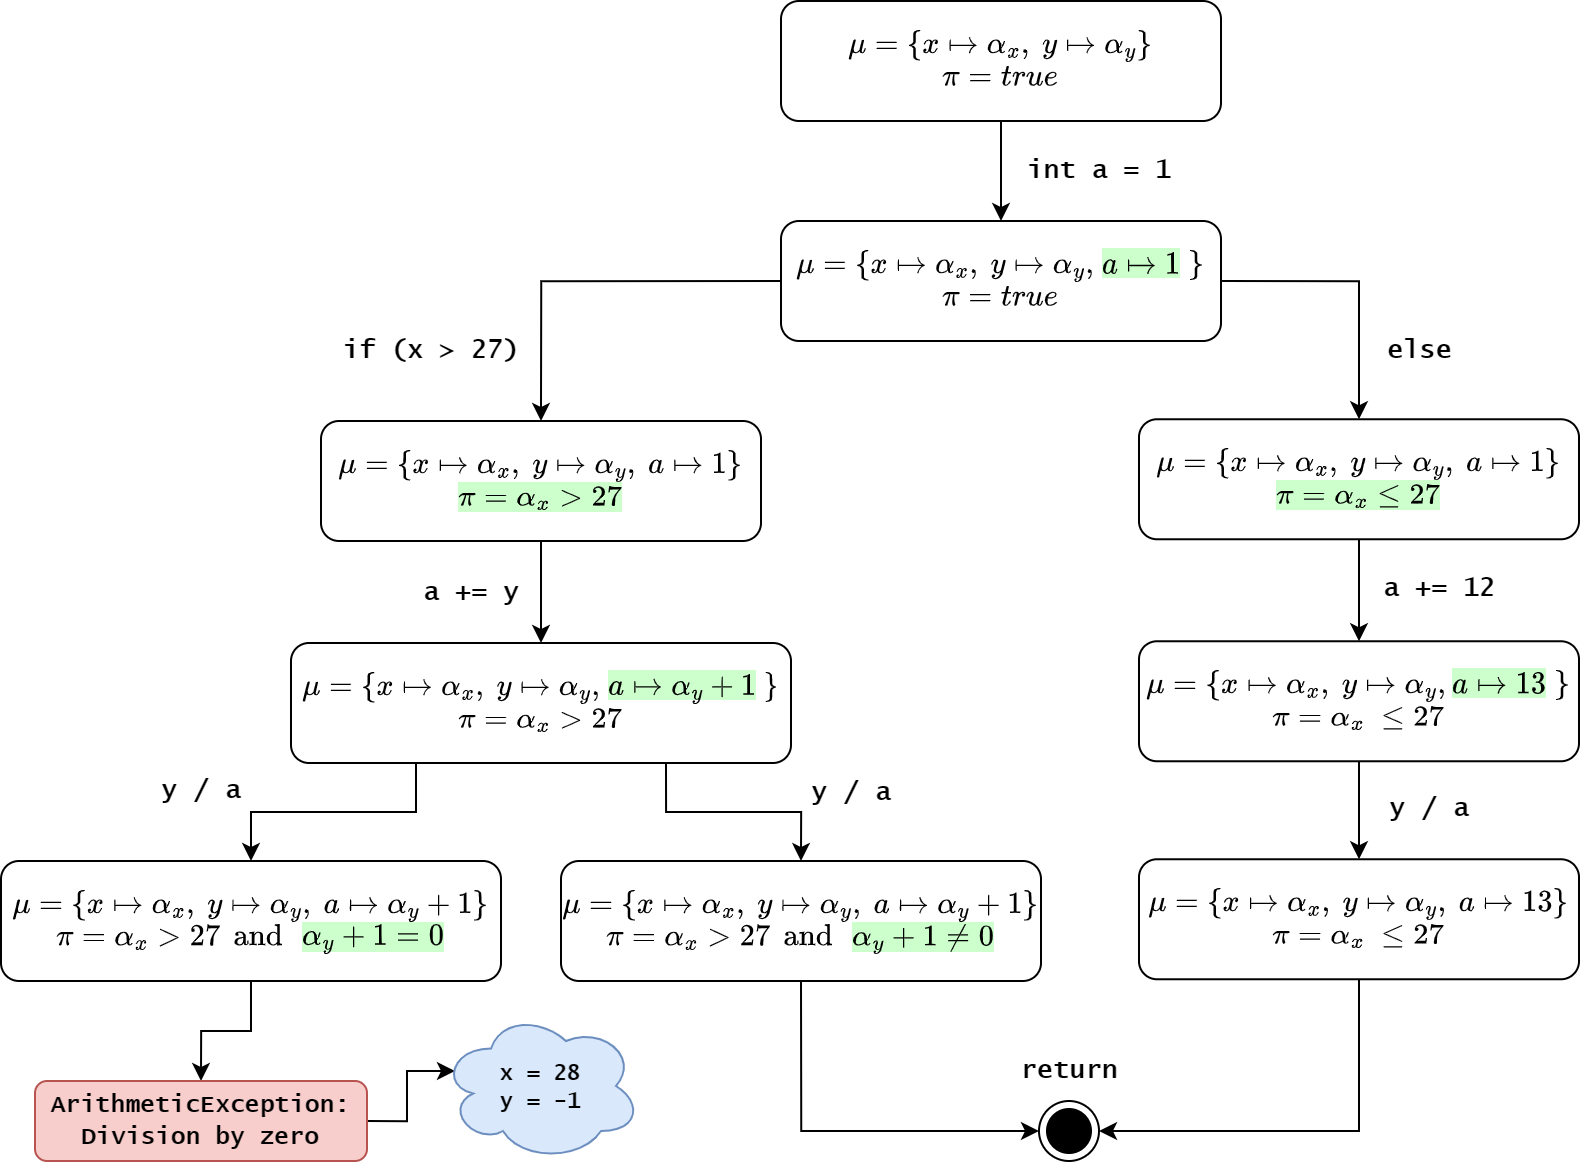
\includegraphics[scale=0.28]{images/se-example-200.png}
    \caption{\label{se-example} Схема символьного исполнения функции \var{example}.}
\end{figure}

По итогам анализа мы хотим ответить на вопрос, существуют ли какие-нибудь конкретные входные аргументы функции \var{example}, при которых в строке 10 выбрасывается исключение \verb|ArithmeticException: / by zero|, и, если существуют, то хотим найти их.

В схеме, представленной на рис. \ref{se-example}, прямоугольник "--- это одно состояние символьной машины. Оно хранит в себе символьную память и условие пути, которые для краткости обозначены $\mu$ и $\pi$ соответственно. Память $\mu$ в данном примере хранит для каждой переменной её символьное значение, то есть для $x$ это $\alpha_x$, а для $y$ "--- $\alpha_y$. Условие пути $\pi$ "--- это логическая формула со значениями символьных переменных, выполняемая на текущем пути исполнения. Переход от состояния к состоянию происходит при обработке некоторой инструкции исходного кода, записанной на соответствующем ребре графа состояний.

Изначально в $\mu$ лежат символьные переменные, на которые ещё не наложено ни одно ограничение, а $\pi$ "--- это всегда выполняющаяся формула, то есть просто $true$.

Обрабатывая инструкции исходного кода, символьная виртуальная машина поддерживает значения $\mu$ и $\pi$ в актуальном состоянии. Например, после строки \verb|int a = 1|, в $\mu$ запомнилась переменная $a$ и её значение $1$. А после обработки условного оператора \verb|if (x > 27)|, исполнение разветвилось на два пути, в каждом из которых обновилось $\pi$: в ветке \verb|if| оно равно $\alpha_x > 27$, а в ветке \verb|else| равно $\alpha_x \le 27$.

В некоторый момент алгоритм обнаруживает состояние, которое ведёт к выбрасыванию исключения. После этого он обращается к SMT-решателю с запросом найти конкретные значения $\alpha_x$ и $\alpha_y$, которые выполняют формулу $\pi = \alpha_x > 27 \land \alpha_y + 1 = 0$, или же сообщить, что решений не существует. В данном примере формула оказывается выполнима, и SMT-решатель возвращает набор $\alpha_x = 28, ~\alpha_y = -1$. Таким образом, удалось автоматически сгенерировать тестовый случай \verb|example(28, -1)|, который приводит к падению программы из-за необработанного исключения.

\newpage

\subsection{UnitTestBot}

UnitTestBot "--- инструмент, который по исходному коду на языке Java автоматически генерирует модульные тесты, пытаясь при этом максимизировать количество покрытых инструкций. UnitTestBot использует для работы собственную символьную виртуальную машину, что даёт возможность ожидать от сгенерированных тестов теоретически полного покрытия кода.

Продукт поставляется как плагин для среды разработки IntelliJ IDEA, что позволяет запускать генерацию тестов, используя удобный пользовательский интерфейс. Инструмент поддерживает популярные системы сборки Gradle и Maven, поэтому его достаточно легко применить на любом проекте, написанном на языке Java. Помимо всего прочего, UnitTestBot предоставляет пользователям множество конфигурируемых параметров своей работы, гибко настраиваясь под нужды тестирования конкретного проекта. В частности, программист может задать количество времени в секундах, которое будет доступно инструменту для генерации тестов.

\subsubsection{Архитектура}\label{sec-utbot-arch}

В данном подразделе будет проведён обзор общей архитектуры проекта, а также некоторых деталей реализации символьной виртуальной машины, которую использует UnitTestBot.

На рис. \ref{utbot-arch} представлена высокоуровневая диаграмма ключевых модулей проекта. 
%Некоторые модули, в особенности те, которые не будут каким-либо образом задействованы или модифицированы в данной работе, не отражены на данной схеме для краткости.
Рассмотрим каждую компоненту подробнее.

\begin{figure}[ht]
    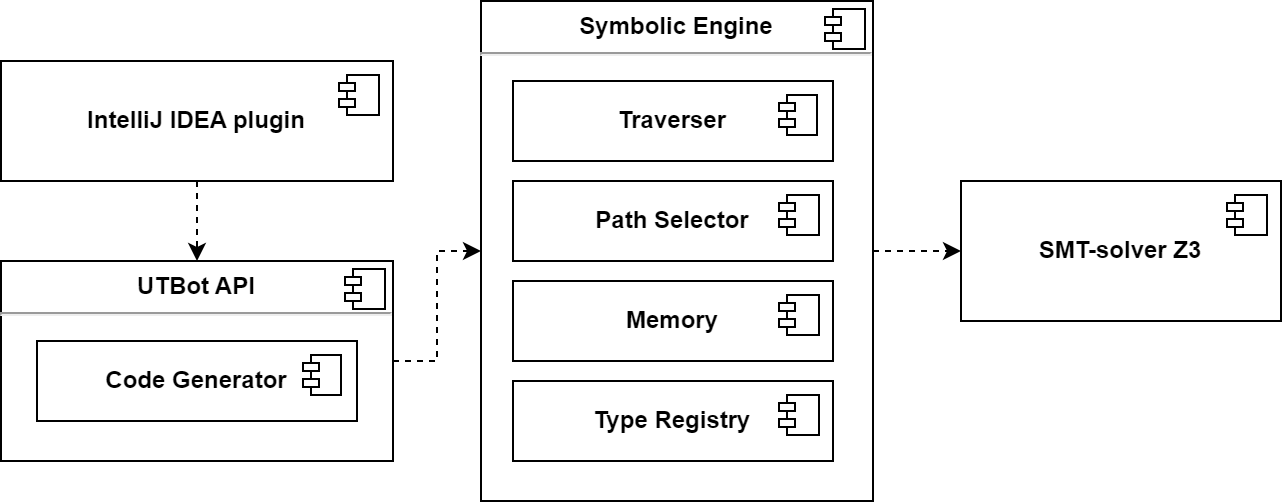
\includegraphics[scale=0.35]{images/utbot-arch-200.png}
    \caption{\label{utbot-arch} Диаграмма основных модулей проекта UnitTestBot.}
\end{figure}

Плагин для IntelliJ IDEA задаёт представление интерфейса в указанной среде разработки. Модуль собирает с пользовательского проекта все нужные для генерации тестов данные, например структуру классов или файлы с Java байт-кодом. Другими словами, является точкой входа в приложение, позволяя настраивать и запускать генерацию тестов.

Пакет \verb|UTBot API| отвечает за формирование входных данных для генерации тестов, запуск символьной виртуальной машины и возвращение результата её работы в удобном для вызывающего кода виде. Типичный сценарий использования данного модуля выглядит следующим образом. Плагин для IntelliJ IDEA совершает запрос на генерацию тестов, передавая байт-код пользовательских классов и все остальные необходимые данные. После чего описываемый компонент преобразует пришедшие данные в нужный формат и запускает на них символьное исполнение. Результат работы символьной машины поступает в \verb|Code Generator|, который генерирует код тестов на языке Java, соответствующий найденным тестовым случаям. В итоге полученный файл с тестами возвращается в модуль плагина и отображается на экране пользователя.

Модуль \verb|Symbolic Engine| "--- это символьная виртуальная машина внутри UnitTestBot, центральный и самый сложный компонент проекта. В качестве входных данных, он ожидает байт-код одного метода\footnote{На самом деле символьная машина работает не с обычным Java байт-кодом, а с упрощённым трёхадресным кодом. Однако для простоты, эта деталь реализации опускается.}, а результатом исполнения является множество тестовых случаев, то есть наборов входных параметров метода. В процессе своей работы модуль делает запросы к SMT-решателю Z3 \cite{z3}, как было описано в общем алгоритме символьного исполнения (в разделе \ref{sec-sym-exec}).

Работа модуля высокоуровнево выглядит следующим образом. На каждом шаге текущее состояние извлекается из \verb|Path Selector|, затем обрабатывается в \verb|Traverser|, который возвращает несколько новых состояний. Для каждого из полученных состояний проверяется, является ли оно терминальным. Если да, то оно запоминается как результат исполнения, а иначе кладётся в очередь состояний внутри \verb|Path Selector|. 

Теперь рассмотрим обязанности наиболее важных классов данного модуля подробнее.

\begin{itemize}
    \item \verb|Path Selector| "--- это класс, принимающий решение о том, какая инструкция программы должна быть обработана следующей. Хранит внутри себя некоторый список доступных состояний (при старте только одно начальное), позволяет добавлять туда новое состояние, а также извлекать некоторое следующее. Какое именно состояние будет извлечено из списка, определяется на основании реализованной внутри эвристики.
    \item \verb|Traverser| обрабатывает поданное на вход состояние. Он содержит информацию о графе потока управления, иерархии классов в программе и системе символьных типов. \verb|Traverser|, в зависимости от состояния и текущей инструкции, создаёт набор новых состояний, в которых обновлена символьная память и добавлены необходимые логические ограничения для соответствующего пути исполнения. Описанное множество состояний и является результатом работы класса.
    \item \verb|Memory| отвечает за символьное представление памяти состояния в программе. Высокоуровнево работает ровно так, как было описано в главе про символьное исполнение (\ref{sec-sym-exec}).
    \item \verb|Type Registry| "--- важный компонент, который содержит информацию о системе типов в анализируемом коде. Даёт возможность узнать тип символьного объекта во время исполнения.
\end{itemize}

\subsubsection{Пример работы}

Рассмотрим пример работы инструмента UnitTestBot на уже знакомой функции \var{example}, которая теперь является методом класса \var{Main}.

\begin{code}
public class Main {

    int example(int x, int y) {
        int a = 1;

        if (x > 27) {
            a += y;
        } else {
            a += 12;
        }

        return y / a;
    }
}
\end{code}

Программист запускает генерацию тестов, используя интерфейс плагина для IntelliJ IDEA, при этом указав количество отведённого на генерацию тестов времени 10 секунд.

Конфигурация, Java байт-код, структура классов, а также вся остальная необходимая информация преобразуется в модуле \verb|UTBot API| и передается в \verb|Symbolic Engine| в ожидаемом для него виде. Тот, в свою очередь, с помощью символьного исполнения находит 2 набора входных параметров функции.
\begin{enumerate}
    \item Набор $x = 27, ~ y = -255$ покрывает все строчки, кроме седьмой, и возвращает $-19$ в качестве результата метода \var{example}.
    \item Набор $x = 28, ~ y = -1$ покрывает оставшуюся непокрытой строку номер 7, а также инициирует выброс необработанного исключения \verb|ArithmeticException: / by zero| в строке 12.
\end{enumerate}

Результат работы \verb|Symbolic Engine| передаётся в \verb|Code Generator|, который для данного примера генерирует следующий код.

\begin{code}
import org.junit.jupiter.api.Test;

import static org.junit.jupiter.api.Assertions.assertEquals;

public final class MainTest {

    @Test
    public void testExample1() {
        Main main = new Main();
        int actual = main.example(27, -255);
        assertEquals(-19, actual);
    }

    @Test
    public void testExample2() {
        Main main = new Main();
        main.example(28, -1);
    }
}
\end{code}

Если запустить полученные тесты, то второй завершится с ошибкой. Это является ожидаемым поведением инструмента, ведь программист забыл обработать возможное исключение. Об этом ему сообщается в виде теста, который не проходит.

\newpage

\subsection{Taint-анализ}

Taint-анализ \cite{taint} "--- это технология, позволяющая отслеживать распространение непроверенных внешних данных по программе. Попадание таких данных в критические секции кода может привести к различным уязвимостям, включая SQL-инъекцию, межсайтовый скриптинг (XSS) и многие другие. Злоумышленники могут использовать эти уязвимости для нарушения корректной работы системы, получения конфиденциальных данных или проведения других несанкционированных операций. Taint-анализ помогает находить описанные ошибки ещё на этапе компиляции. Отметим, что методика может быть применена и во время непосредственного выполнения программы \cite{dyn-taint}, однако данная работа не будет затрагивать эту область.

\subsubsection{Описание алгоритма}

Ключевая идея подхода заключается в том, что любая переменная, которая может быть изменена внешним пользователем, представляет потенциальную угрозу безопасности. Если эта переменная используется в некотором выражении, то значение этого выражения также становится подозрительным. Далее, алгоритм отслеживает и оповещает о ситуациях, когда какая-либо из этих \textit{помеченных} переменных используется для выполнения опасных команд, например, прямых запросов в базу данных или в операционную систему компьютера.

Для своей работы, taint-анализ требует конфигурацию, в которой методам программы можно назначить одну из следующих ролей.

\begin{itemize}
    \item \verb|Taint source| "--- \textit{источник} непроверенных данных. К примеру, это может быть метод считывания пользовательского ввода или же метод получения параметра пришедшего HTTP-запроса. Переменные, в которые записывается результат выполнения \verb|Taint source|, называются \textit{помеченными}. Семантика метода определяет, какая именно метка будет наложена на переменную. Причём имя метки может быть совершенно произвольным, так как его выбирает тот, кто пишет конфигурацию. \\
    Например, может быть задано, что функция \verb|getPassword()| накладывает метку \verb|"sensitive-data"| на своё возвращаемое значение.
    \item \verb|Taint sink| "--- \textit{приёмник}, некоторая критическая секция приложения. Это может быть метод прямого обращения к базе данных или файловой системе, а также любая другая потенциально опасная операция. Для \verb|Taint sink| можно задать набор меток, переменные с которыми не должны в него просочиться. \\
    К примеру, если значение с меткой \verb|"sensitive-data"| передаётся в функцию журналирования, которая печатает свои аргументы напрямую в консоль, то это ошибка разработчика, так как происходит утечка данных.
\end{itemize}

Помимо источников и приёмников, есть ещё две вспомогательные сущности, которые нужны для расширения возможностей алгоритма.
\begin{itemize}
    \item \verb|Taint pass| "--- это функция, которая помечает возвращаемое значение с учётом меток в её аргументах. В зависимости от реализации, метки могут накладываться не только на результат метода, но и на объект \verb|this|, и на входные параметры. \\
    Например, в конфигурации может быть установлено, что метод конкатенации строк \verb|concat(String a, String b)| помечает свой результат всеми метками из \var{a} и из \var{b}.
    \item \verb|Taint cleaner| "--- это функция, которая удаляет заданный набор меток из переданных аргументов. Чаще всего, это некоторый метод валидации, который проверяет, что пользователь ввёл данные в ожидаемом формате. \\
    К примеру, метод \verb|validateEmail(String email)| удаляет метку \verb|XSS| при успешном прохождении проверок, так как теперь в строке \var{email} точно нет непроверенных данных, которые могут привести к уязвимости межсайтового скриптинга.
\end{itemize}

Алгоритм taint-анализа сканирует граф потока данных, пытаясь обнаружить маршрут между методом из множества \verb|Taint sources| и методом из \verb|Taint sinks|. Основной проблемой классического алгоритма, как и у всех методов неточного анализа, является большое количество ложноположительных срабатываний. Однако существуют научные публикации \cite{sym-taint}, в которых данная проблема решается с помощью применения символьного исполнения. Другими словами, если встроить taint-анализ непосредственно внутрь символьной виртуальной машины, то удаётся практически полностью избавиться от ложных результатов, а также заодно получить конкретные входные данные, реализующие найденный путь от источника к приёмнику. Последний подход и будет реализован в данной работе.

\subsubsection{Пример работы}

Рассмотрим пример простой функции, в которой есть уязвимость вида SQL-инъекция: если злоумышленник введёт в переменную \var{name} строку \verb|"name'); DROP TABLE Employees; --"|, то у него получится удалить таблицу \verb|Employees| вместе со всеми данными, которые в ней хранились.

\begin{code}
void example(Connection connection) throws SQLException {
    Scanner sc = new Scanner(System.in);
    String name = sc.nextLine();

    Statement stmt = connection.createStatement();
    String query = 
        "INSERT INTO Employees(name) VALUES('"
        .concat(name)
        .concat("')");
    stmt.executeUpdate(query);
}
\end{code}

Для работы taint-анализа нужно сначала задать правильную конфигурацию.
\begin{itemize}
    \item \verb|Taint source| "--- метод \verb|nextLine| класса \verb|java.util.Scanner|, который добавляет к возвращаемому значению метку \verb|"user-input"|.
    \item \verb|Taint pass| "--- метод \verb|concat| класса \verb|java.lang.String|, который пропускает через себя метку \verb|"user-input"|, полученную либо у первого аргумента, либо у объекта, на котором этот метод вызывается (то есть у \verb|this|).
    \item \verb|Taint sink| "--- метод \verb|executeUpdate| класса \verb|java.sql.Statement|, который отслеживает переменные, помеченные \verb|"user-input"|.
\end{itemize}

Любая корректная реализация taint-анализа должна найти в этом коде ошибку: переменная \var{query} с меткой \verb|"user-input"| передаётся в приёмник \verb|executeUpdate|. 

Важно отметить, что в обязанности алгоритма не входит нахождение конкретных данных, которые бы смог ввести злоумышленник, чтобы навредить программе. Требуется лишь обнаружить маршрут, соединяющий источник и приёмник.

\section{Создание отчёта по сгенерированным тестам}

Результатом работы любого статического анализатора является некоторый отчёт. Иначе говоря, список обнаруженных ошибок вместе со всей дополнительной информацией, которая может помочь программисту разобраться в проблеме быстрее.

Таким образом, первая задача, которая решается в данной работе "--- создание такого отчёта по имеющимся данным, а именно по сгенерированным инструментом UnitTestBot тестам. Причём наибольший интерес вызывают тестовые случаи, приводящие к падению программы, то есть к выбрасыванию необработанных исключений. Следовательно, сообщение об ошибке должно содержать конкретное место в коде, где возникает исключение, а также путь исполнения, который к нему приводит.

\subsection{Формат SARIF}

В качестве формата отчёта был выбран SARIF (Static Analysis Results Interchange Format) \cite{sarif}. Это формат на основе JSON \cite{json}, созданный специально для единообразного описания результатов статического анализа. Принят как стандарт OASIS\footnote{Organization for the Advancement of Structured Information Standards) "--- глобальный консорциум, который управляет разработкой, конвергенцией и принятием промышленных стандартов электронной коммерции в рамках международного информационного сообщества.} и используется во многих популярных инструментах.

Рассмотрим структуру формата, а также основные возможности для описания ошибок, которые он предоставляет. Легче всего это сделать на примере небольшого отчёта, который приведён ниже (для краткости все незначащие детали заменены на многоточие).

\begin{zerocode}
{
  "schema" : "https://.../sarif-schema-2.1.0.json",
  "version" : "2.1.0",
  "runs" : [
    "tool" : { ... },
    "results" : [ {
      "ruleId" : "...",
      "level" : "error",
      "message" : { "text" : "..." },
      "locations" : [ ... ],
      "relatedLocations" : [ ... ],
      "codeFlows" : [ ... ]
    } ]
  ]
}
\end{zerocode}

На самом верхнем уровне формат определяет \var{runs} "--- список результатов различных запусков анализатора.

Каждый запуск содержит в себе \var{tool} "--- некоторая информации об инструменте и \var{results} "--- непосредственно список обнаруженных ошибок.

Один результат описывается ключами 

\begin{itemize}
    \item \var{ruleId} "--- уникальный идентификатор для данного типа ошибки.
    \item \var{level} "--- уровень серьезности дефекта, например, \verb|error| или \verb|warning|.
    \item \var{message} "--- сообщение, которое будет показано пользователю.
    \item \var{locations} "--- список мест в коде, где была найдена ошибка. Каждый отдельный \var{location} имеет собственное внутреннее устройство, о котором рассказано ниже.
    \item \var{relatedLocations} "--- список мест в коде, каким-либо образом связанных с ошибкой. Элементами списка являются те же объекты \var{location}.
    \item \var{codeFlows} "--- список путей, по которым прошла программа, прежде чем наткнуться на обнаруженный дефект.
\end{itemize}

Объект \var{location} состоит из пути до файла \var{artifactLocation} и позиции внутри файла \var{region}. Пример объекта \var{location} представлен ниже.

\begin{zerocode}
"physicalLocation" : {
  "artifactLocation" : {
    "uri" : "src/examples/Main.java"
  },
  "region" : {
    "startLine" : 91,
    "startColumn" : 9,
    "endLine": 91,
    "endColumn": 20
  }
}
\end{zerocode}

Как уже отмечалось ранее, SARIF имеет неплохую поддержку в сфере анализа программ. В частности, смотреть отчёт в удобном виде, с навигацией по коду и другими полезными функциями, можно в редакторе Visual Studio Code \cite{vscode}. Также есть интеграция с CI/CD платформы GitHub \cite{sarif-git}, что может быть удобно для больших команд разработчиков.

\subsection{Извлечение информации из тестов}

Теперь опишем, как именно разработанный модуль формирования отчётов получает нужную информацию об ошибках по результатам символьного исполнения.

После того как UnitTestBot отработал на пользовательском коде и сгенерировал для него тесты, модуль смотрит на набор найденных терминальных состояний, другими словами, на тестовые случаи. При этом он будет рассматривать только те состояния, которые приводят к выбрасыванию исключения.

В терминальном состоянии \var{state} содержится достаточно много полезной информации. Во-первых, в там хранится результат исполнения, в нашем случае это тип возникающего исключения. Во-вторых, конкретные входные данные анализируемого метода, полученные из SMT-решателя. Зная это, модуль формирует сообщение об ошибке по шаблону ниже.

\begin{zerocode}
"Unexpected ArithmeticException: / by zero.
 Test case: example(28, -1)."
\end{zerocode}

В данном случае было найдено деление на ноль при запуске метода \var{example} с аргументами $28$ и $-1$.

В \var{state} также содержится путь из инструкций \var{path}, по которому машина пришла в это состояние. Она работает с трёхадресным Java байт-кодом, однако внутри UnitTestBot есть механизм, который по любой инструкции может вернуть номер соответствующей строчки в исходном коде.

Чтобы восстановить номер строки с ошибкой \var{startLine}, достаточно взять последний элемент из списка \var{path}. Далее, модуль считывает строку с номером \var{startLine} из файла с кодом пользователя и вычисляет \var{startColumn} и \var{endColumn}, обрезая пробельные символы с начала и с конца. Таким образом, формируется поле \var{location} в отчёте.

Поле \var{codeFlows} также восстанавливается из значения \var{path}. Модуль анализирует граф вызовов методов на пути \var{path} и назначает для каждого уровня вложенности последнюю на этом уровне инструкцию. Полученный список номеров строк оказывается равен настоящей трассировке стека, как если бы мы просто запустили код с найденными входными аргументами, то есть ровно то, что и требовалось.

Последнее, что фиксируется в отчёте "--- это поле \var{relatedLocations}. В него помещается ссылка на соответствующий данному результату тест в файле со сгенерированными тестами. Когда стартует разработанный модуль, UnitTestBot уже записал тесты в выходной файл, а значит можно просто найти позицию нужного теста по его имени в этом файле.

В итоге вся собранная информация структурируется и сериализуется в JSON.

% можно ещё добавить про минимизацию результатов

\subsection{Пример работы}

Модуль поддерживает все стандартные исключения Java, в том числе и \verb|AssertionError|, поэтому, один из типичных способов использования инструмента выглядит следующим образом. Программист сначала расставляет \verb|assert| проверки в коде, если хочет гарантировать выполнение некоторых инвариантов. После чего он запускает разработанный статический анализатор, который выявляет все места, где проверки не проходят.

Рассмотрим пример его работы на функции \var{abs}, которая, как понятно из названия, должна возвращать модуль числа. Её возвращаемое значение обязано быть не меньше нуля, и, чтобы это гарантировать, в методе присутствует строчка \verb|assert x >= 0|.

\begin{code}
public class Main {
    int abs(int x) {
        if (x < 0) {
            x *= -1;
        }
        assert x >= 0;
        return x;
    }
}
\end{code}

Однако UnitTestBot обнаружил, что передача числа $-2^{32}$ приводит к \verb|AssertionError| (происходит переполнение типа \verb|int|), что и отражено в сформированном отчёте SARIF. Он получился достаточно большим (около 100 строк), поэтому для краткости я перечислю в здесь только значения важных полей без сохранения структуры формата SARIF.

\begin{itemize}
    \item Сообщение об ошибке:

\begin{zerocode}
"message" : {
  "text" : "Unexpected AssertionError.
            Test case: abs(-2147483648)"
}
\end{zerocode}

    \item Местоположение ошибки:

\begin{zerocode}
"uri" : "src/Main.java",
"region" : {
  "startLine" : 6,
  "startColumn" : 9
}
\end{zerocode}

    \item Местоположение сгенерированного теста:

\begin{zerocode}
"uri" : "utbot_tests/MainTest.java",
"region" : {
  "startLine" : 29,
  "startColumn" : 5
}
\end{zerocode}

    \item Трассировка стека:

\begin{zerocode}
[
    "MainTest.testAbs3(MainTest.java:34)",
    "Main.abs(Main.java:6)"
]
\end{zerocode}

\end{itemize}

\section{Плагин для IntelliJ IDEA}

Абсолютное большинство программистов используют различные интегрированные среды разработки. Ключевой особенностью современных IDE является возможность подключения в них плагинов "--- сторонних модулей, выполняющих определённые задачи. Таким образом, каждый пользователь может установить себе нужный набор плагинов и решать возникающие при программировании задачи прямо в IDE, что часто удобнее, чем пользоваться отдельными сервисами.

Многие статические анализаторы имеют собственные плагины под ту или иную среду разработки. В данной работе было принято решение реализовать плагин для IntelliJ IDEA, который бы позволял запускать статический анализ и просматривать его результаты, то есть отчёт SARIF. Разработка, однако, велась не с нуля, а на основе уже существующего плагина для автоматической генерации модульных тестов "--- UnitTestBot.

\subsection{Детали реализации}

Платформа IntelliJ предоставляет сторонним разработчикам широкие возможности по созданию новых модулей \cite{idea-plugins}. В частности, существует стандартный механизм \verb|Inspections|, который позволяет отображать список найденных проблем на панели \verb|Problems View|. Для того чтобы воспользоваться этой возможностью, были выполнены следующие шаги.

\begin{enumerate}
    \item Зарегистрирован новый \verb|InspectionTool| в конфигурации плагина.
    \item Переопределён метод \verb|GlobalSimpleInspectionTool.checkFile|, который добавляет обнаруженные ошибки для конкретного переданного файла \var{psiFile} в общий список проблем для \var{psiFile}.
    \item Добавлен автоматический запуск механизма \verb|Inspections| сразу после генерации тестов и создания отчёта SARIF, чтобы отобразить найденные дефекты в IDE.
\end{enumerate}

Ниже представлен сценарий использования модифицированного плагина.

\begin{enumerate}
    \item Пользователь запускает генерацию тестов в специальном режиме, который предполагает дальнейшее отображение результатов статического анализа.
    \item После окончания работы символьной машины и создания отчёта SARIF, на экране открывается вкладка \verb|Problems View|, где перечислены обнаруженные инструментом ошибки и уязвимости в виде списка сообщений (поле \var{message} в SARIF).
    \item При нажатии на любой из элементов этого списка, IDE показывает соответствующую ему строчку кода (поле \var{location}).
    \item В окошке справа появляется кнопка для перехода к нужному сгенерированному тесту (поле \var{relatedLocation}).
    \item Также, есть возможность посмотреть трассировку стека найденного исключения (поле \var{codeFlows}). Причём эта функциональность поддерживает навигацию по коду для каждого представленного кадра стека.
\end{enumerate}

Отдельно отметим, что перед разработкой самого интерфейса, было исследовано несколько альтернативных путей решения задачи по визуализации результатов. Например, для этого можно было написать отдельный плагин или сверстать собственную вкладку. В итоге было решено, что способ с использованием уже готовых \verb|Inspections| и \verb|Problems View| будет наиболее прост в реализации и, при этом, привычен для конечного пользователя, поэтому был выбран именно он.

Помимо описанной функциональности, плагин имеет дополнительные возможности для повышения удобства использования. Например, существует возможность запускать анализ не только на одном выбранном классе, но и на нескольких, а также на всём проекте сразу.

\subsection{Пример работы}

В приложении на Рис. \ref{problems-view} представлен снимок экрана среды IntelliJ IDEA с разработанным пользовательским интерфейсом визуализации результатов статического анализа. В данном случае, инструмент был запущен на методах \var{Main.example} и \var{Util.abs}, реализации которых уже появлялись в примерах ранее, а также на методе \var{Main.sumAbs}.

\begin{code}
int sumAbs(int a, int b) {
    return Util.abs(a) + Util.abs(b);
}
\end{code}

При нажатии на кнопку \verb|View generated test|, происходит переход к соответствующему тесту, как показано в приложении на Рис. \ref{problems-view-test}. 

При нажатии на кнопку \verb|Analyze stack trace|, открывается вкладка, представленная в приложении на Рис. \ref{problems-view-stacktrace}.

\section{Taint-анализ}

Как уже было упомянуто, taint-анализ позволяет находить уязвимости в безопасности, отслеживая распространение непроверенных пользовательских данных по программе. Алгоритм действительно очень известный, ведь те или иные его модификации реализованы во многих популярных анализаторах. В частности, в некоторых из тех, что были рассмотрены во введении.

Одной из задач данной работы является реализация taint-анализа поверх символьной виртуальной машины UnitTestBot, что избавит описываемую технику от ложноположительных срабатываний. Таким образом, в результате модификации, единственным источником неточностей останется только само символьное исполнение.

\subsection{Конфигурация}

В процессе изучения темы не было найдено ни одного универсального формата конфигурации taint-анализа, а все известные мне статические анализаторы описывают свой собственный способ настройки. Таким образом, первая подзадача, которую нужно было решить ещё до модификации ядра символьной машины, "--- придумать схему конфигурации, где бы можно было описать правила (\verb|sources|, \verb|passes|, \verb|cleaners| и \verb|sinks|), с которыми будет вестись работа в дальнейшем. Формат должен быть удобен для пользователя, но в то же время предоставлять достаточно широкие возможности по настройке алгоритма. Исходя из перечисленных требований, в качестве базового языка разметки был взят YAML \cite{yaml}.

Теперь рассмотрим созданный формат в подробностях. Общая структура конфигурационного документа представлена ниже.

\begin{nocode}
sources:
  - <rule-1>
  - <rule-2>
  - < ... >
passes: [ ... ]
cleaners: [ ... ]
sinks: [ ... ]
\end{nocode}

То есть это просто списки правил, относящиеся к конкретному типу. Каждое правило имеет некоторый набор характеристик.

\begin{itemize}
    \item Уникальный идентификатор метода, которого описывает данное правило. Состоит из полного имени метода, включающего имя пакета и имя класса, а также из сигнатуры метода "--- набора типов его аргументов (ключ \verb|signature| в YAML).
    \item Некоторые условия \verb|conditions|, которые должны выполняться во время исполнения, чтобы правило сработало.
    \item Множество меток \verb|marks|, которыми оперирует правило.
    \item Набор конкретных действий по управлению метками, которые происходят при срабатывании правила (\verb|add-to|, \verb|get-from|, \verb|remove-from| или \verb|check| в зависимости от семантики правила).
\end{itemize}

Таким образом, одно правило, например \verb|taint source|, может выглядеть следующим образом.

\begin{nocode}
com.abc.ClassName.methodName:
  signature: [ <int>, _, <java.lang.Object> ]
  conditions:
    arg1: 
      not: [ -1, 1 ]
  add-to: [ this, arg2, return ]
  marks: user-input
\end{nocode}

Данное правило определяется для метода с именем \var{methodName} из класса \var{ClassName}, который находится в пакете \verb|com.abc|. Метод принимает ровно $3$ аргумента, первый из которых имеет тип \var{int}, второй может быть совершенно любым, а последний имеет тип \verb|java.lang.Object|. Ключ \var{signature} может быть не указан, тогда подходящей считается любая перегрузка \var{methodName}.

Срабатывание происходит только в том случае, когда первый аргумент (\var{arg1}) не равен ни $-1$, ни $1$ , что и указано по ключу \var{conditions} (список интерпретируется как логическое ИЛИ). Данный параметр является необязательным, в случае его отсутствия не будут проверены никакие условия. 

Описанный источник накладывает метку \verb|user-input| к переменным, соответствующим \var{this}, \var{arg2} и \var{return}. Другими словами, к объекту класса \var{ClassName}, на котором вызывается \var{methodName}, второму аргументу функции и возвращаемому значению. Причём по ключам \verb|add-to| и \var{marks} может лежать как список, так и одиночное значение "--- это сделано для удобства использования.

Остальные типы правил имеют такой же синтаксис, как и \verb|source|, за исключением ключа \verb|add-to|.

\begin{itemize}
    \item \verb|Taint pass| передаёт метки с одного множества объектов на другое, поэтому для него определяются два ключа: \verb|get-from| и \verb|add-to| соответственно. Причём на \verb|add-to| накладываются все указанные в \verb|marks| метки, если в \verb|get-from| есть хотя бы одна из них.
    \item \verb|Taint cleaner| удаляет метки с множества объектов, поэтому его ключ называется \verb|remove-from|.
    \item \verb|Taint sink| проверяет наличие некоторых меток в переменных, множество которых лежит по ключу \verb|check|.
\end{itemize}

Разработанный формат, с одной стороны, является лаконичным и читабельным для конечного пользователя, а с другой стороны, достаточно мощным для описания сложных правил или условий срабатывания.

Для описанной схемы конфигурации был реализован парсер, а также произведена необходимая интеграция с плагином для IntelliJ IDEA, чтобы программист мог настраивать taint-анализ под свой конкретный проект. 

Итоговый инструмент можно применять, и не составляя новых правил, для этого были добавлены распространённые источники и приёмники непроверенных данных. Приведём примеры для ясности. 

\begin{itemize}
    \item \verb|java.util.Scanner.nextLine| "--- это \verb|source|, накладывающий метку \verb|user-input| на возвращаемое значение.
    \item \verb|java.lang.String.concat| "--- это \verb|pass|, который добавляет к возвращаемому значению все метки, полученные из \verb|this| и \verb|arg1|.
    \item \verb|java.lang.String.isEmpty| "--- это \verb|cleaner|, который удаляет все метки из объекта \verb|this| в том случае, если \verb|return| равняется \verb|true| (пустая строка не может содержать вредоносных данных).
    \item \verb|java.sql.Statement.execute| "--- это \verb|sink| для меток \verb|user-input|.
\end{itemize}

\subsection{Детали реализации}

В данном подразделе будут описаны общие концепции интеграции taint-анализа и символьного исполнения, а также детали реализации в UnitTestBot.

\subsubsection{Общие концепции}

Ключевая идея состоит в том, чтобы для каждой символьной переменной поддерживать набор меток, наложенных на неё в процессе работы символьной машины (подробнее о символьном исполнении описано в разделе \ref{sec-sym-exec}). Эти наборы могут изменяться только при вызове метода, для которого существует правило в конфигурации (\verb|source|, \verb|pass|, \verb|cleaner| или \verb|sink|). 

Общий вид обработки источника представлен в алгоритме \ref{source-algo}. Для каждого заданного в конфигурации правила \verb|rule|, которое относится к текущему методу, и для каждой сущности \verb|entity| внутри него (\verb|this|, \verb|return| или аргумент метода) алгоритм получает соответствующую ему символьную переменную \verb|symbol|, после чего добавляет к её набору меток \verb|marks[symbol]| метки из \verb|rule|.

\begin{algorithm}[hbt!]
\caption{Обработка источника помеченных данных}\label{source-algo}

\SetKwProg{ProcessTaintSource}{ProcessTaintSource}{}{}
\ProcessTaintSource{$(config, stmt)$}{
    \KwData{$config$ "--- набор правил taint-анализа}
    \KwData{$stmt$ "--- текущая инструкция (вызов метода)}
    
    $rules = config.getSourcesBy(stmt)$\;
    \ForEach{$rule \in rules$}{
        \ForEach{$entity \in rule.entities$}{
            $symbol \gets getSymbolicValue(stmt, entity)$\;
            $marks[symbol] = marks[symbol] \cup rule.marks$\;
        }
    }
}
\end{algorithm}

Алгоритм обработки правил \verb|taint sink| (\ref{sink-algo}) выглядит также, с той лишь разницей, что вместо добавления символьная машина проверяет наличие запрещённых меток \verb|rule.marks| во множестве \verb|marks[symbol]|, и, если пересечение множеств не пусто, то сообщает о найденной уязвимости.

\begin{algorithm}[hbt!]
\caption{Обработка приёмника помеченных данных}\label{sink-algo}

\SetKwProg{ProcessTaintSink}{ProcessTaintSink}{}{}
\ProcessTaintSink{$(config, stmt)$}{
    \KwData{$config$ "--- набор правил taint-анализа}
    \KwData{$stmt$ "--- текущая инструкция (вызов метода)}
    
    $rules = config.getSinksBy(stmt)$\;
    \ForEach{$rule \in rules$}{
        \ForEach{$entity \in rule.entities$}{
            $symbol \gets getSymbolicValue(stmt, entity)$\;
            \If{$marks[symbol] \cap rule.marks \neq \varnothing $}{
                $reportProblem()$\;
            }
        }
    }
}
\end{algorithm}

Алгоритмы для правил \verb|taint pass| и \verb|cleaner| аналогичны представленным выше, за исключением строки с изменением \verb|marks| (в соответствии со своей семантикой), поэтому для краткости в тексте работы не приводятся.

\subsubsection{Модификация символьной машины}

Теперь подробно рассмотрим детали встраивания taint-анализа в выбранную символьную виртуальную машину.

Общий вид работы UnitTestBot выглядит следующим образом. На вход инструменту поступает программа в виде инструкций байт-кода. Объект \verb|PathSelector| определяет порядок обхода символьных состояний, \verb|Traverser| отвечает за обработку одной инструкции, а также поддерживает символьную память \verb|Memory| и систему типов \verb|TypeRegistry| в актуальном виде. В терминальном состоянии делается запрос к SMT-решателю с целью определить выполнимость пройденного пути и найти для него конкретные входные данные. Более подробное описание ключевых мест в процессе работы UnitTestBot представлены в разделе \ref{sec-utbot-arch}.

Основная идея реализованного подхода состоит в том, что каждой символьной переменной сопоставляется \verb|taint vector| "--- 64-битное значение, каждый бит \var{i} которого отвечает за наличие метки с номером \var{i} в этом объекте. После чего, в процессе работы символьной машины, эти сопоставления поддерживаются и обновляются в соответствии с классическим алгоритмом taint-анализа.

Сделанные в данной работе изменения в большинстве своём затрагивают классы \verb|Traverser| и \verb|Memory|. Также, были добавлены новые компоненты \verb|TaintModel|, \verb|TaintMarkRegistry| и \verb|TaintMarkManager|. На рис. \ref{taint-arch} представлена высокоуровневая диаграмма разработанного модуля. Разберём зону ответственности каждой сущности подробнее.

\begin{figure}[ht]
    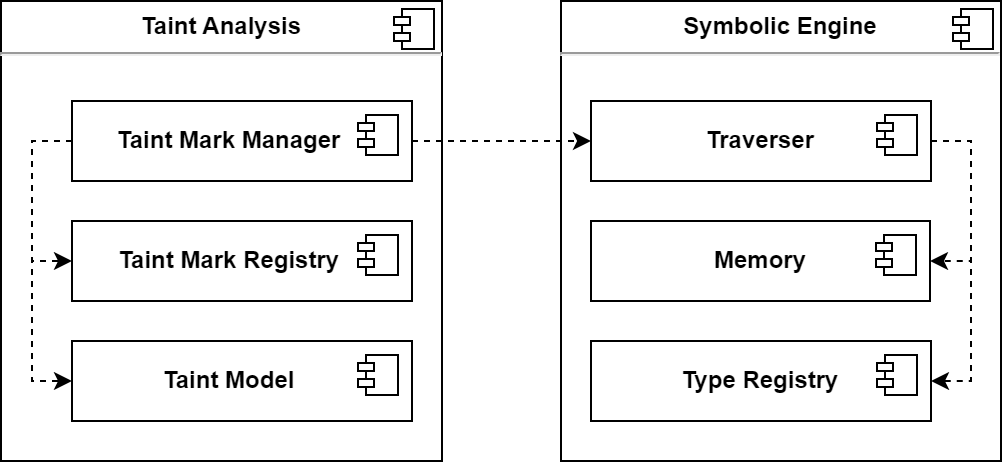
\includegraphics[scale=0.35]{images/taint-arch-tr-200.png}
    \centering\caption{\label{taint-arch} Архитектура модуля Taint-анализа.}
\end{figure}

Объект класса \verb|TaintMarkRegistry| хранит сопоставление между именем метки и её порядковым номером от $0$ до $63$. Видим, что количество меток, которые могут быть одновременно задействованы в анализе, ограничено числом $64$. Однако, во-первых, этого хватает для почти любого разумного примера, а во-вторых, решение было обусловлено вопросами производительности "--- операции с типом данных \verb|Long| совершаются намного быстрее, чем если бы был использован битовый массив произвольного размера. 

Компонент \verb|TaintModel| отвечает за предоставление доступа к конфигурации. В частности, он определяет способ преобразования условий (значение по ключу \verb|conditions| в YAML-документе) в логические выражения над символьными переменными. Отметим, что сам \verb|TaintModel| не выполняет никаких действий, а лишь предоставляет процедуру, которую можно запустить, уже имея на руках \verb|Memory| и \verb|TypeRegistry|.

\verb|Memory| занимается хранением значений \verb|taint vector| для символьных переменных. В этом же классе были реализованы простые функции для обновления векторов и их получения по адресу символьного объекта. Вся сложная логика по добавлению и удалению меток, опирающаяся на теорию taint-анализа, была написана в отдельной сущности \verb|TaintMarkManager|. Другими словами, этот класс оборачивает низкоуровневую работу с памятью в понятные с точки зрения предметной области операции.

Обновление информации о помеченных переменных происходит в процессе работы \verb|Traverser|. Перед каждой из \verb|invoke| инструкций, которые соответствуют запуску некоторого метода в пользовательском коде, вызывается специальный обработчик \verb|processTaintSink|, а уже после инструкции \verb|invoke| вызываются обработчики \verb|processTaintSource|, \verb|processTaintPass| и \verb|processTaintCleaner|. Такой порядок связан с тем, что всем правилам, кроме приёмников, нужен результат работы функции. При этом факт передачи заражённых данных происходит в момент запуска функции-приёмника, поэтому сообщить о найденной уязвимости можно ещё до её выполнения. 

Перечисленные обработчики правил обращаются к \verb|TaintModel|, чтобы проверить, есть ли информация про рассматриваемый метод в конфигурации, и, если есть, то получить её. Функция \verb|processTaintSink| запрашивает у \verb|TaintMarkManager| данные об уже выставленных метках и добавляет ограничения в SMT-решатель, выполнение которых соответствует обнаружению дефекта. Остальные обработчики изменяют символьную память \verb|Memory| через тот же \verb|TaintMarkManager|, добавляя и удаляя метки у выбранных символьных объектов.

В результате удаётся не только обнаружить возможные уязвимости, но и сгенерировать конкретные входные данные, запуск программы на которых покажет, по какому маршруту заражённые переменные могут проникнуть в критические секции кода.

\subsubsection{Модификация генератора кода}

Результатом работы UnitTestBot, помимо добавленного в данной работе отчёта SARIF, являются тесты. Другими словами, на каждом найденном тестовом случае запускается \verb|CodeGenerator|, который должен оформить тест в виде кода на языке Java. Причём, если тест ведёт к выбрасыванию необработанного исключения, то он не должен проходить.

Ошибки, которые получаются в результате работы модуля taint-анализа, не являются настоящими с точки зрения языка, так как это не исключения. Однако хотелось бы всё равно выделить такие тесты как провальные, поэтому генератор кода был изменён таким образом, чтобы в конце каждого теста добавлялась искусственная ошибка, которая бы и обеспечивала падение.

\begin{code}
Assertions.fail(
    "'java.lang.String' marked 'user-input'
     was passed into 'Statement.execute' method"
);
\end{code}

Предоставленное решение оказалось очень удачным, ведь оно позволило автоматически получить интеграцию с отчётами SARIF и визуализацией результатов во вкладке \verb|Problems view| в IntelliJ IDEA. Найденный тестовый случай теперь трактуется как настоящее исключение, а для них уже написана вся нужная логика.

\subsection{Пример работы}

Рассмотрим пример работы реализованного модуля на классе \verb|User|. 

\begin{code}
public class User {

    String getLogin() { /* some logic */ }

    String getPassword() { /* some logic */ }

    String userInfo(String login, String password) {
        return login + "#" + password;
    }

    void printUserInfo() {
        var login = getLogin();
        var password = getPassword();
        var info = userInfo(login, password);
        System.out.println(info);
    }
}
\end{code}

Метод \verb|getPassword| возвращает чувствительные данные, которые ни в коем случае не должны утечь из приложения, а программист печатает их в стандартный поток вывода, что является серьёзной ошибкой.

Сначала напишем конфигурацию, которая выражает сказанную мысль, и сохраним её в файл \verb|./.idea/utbot-taint-config.yaml|, откуда её сможет прочесть анализатор.

\begin{nocode}
sources:
  - User.getPassword:
      add-to: return
      marks: sensitive-data
passes:
  - User.userInfo:
      get-from: [ arg1, arg2 ]
      add-to: return
      marks: [] # all
sinks:
  - java.io.PrintStream.println:
      check: arg1
      marks: sensitive-data
\end{nocode}

Теперь запускаем UnitTestBot с помощью плагина для IntelliJ IDEA и смотрим на полученный результат.

Во-первых, сгенерировался тест, по которому понятно, что модуль taint-анализа нашёл уязвимость.

\begin{code}
@Test
public void testPrintUserInfo1() {
    User user = new User();
    user.printUserInfo();
    fail(
        "'java.lang.String' marked 'sensitive-data' 
         was passed into 'PrintStream.println' method"
    );
}
\end{code}

Во-вторых, появилась панель \verb|Problems view| (рис. \ref{problems-view-taint}), где отображена найденная проблема в виде результата статического анализа.

Разберём чуть подробнее внутренности работы модуля на данном примере.

После выполнения метода \verb|getPassword| символ, соответствующий переменной \verb|password|, помечается как \verb|sensitite-data| (возводится нулевой бит в его \verb|taint vector|).

После вызова \verb|userInfo| помечается также переменная \verb|info|, так как \verb|userInfo| "--- это \verb|taint pass|, который добавляет к возвращаемому значению все метки, собранные из обоих своих аргументов.

Перед печатью \verb|info| на консоль, функция-обработчик \verb|processTaintSink| добавляет ограничение в SMT-решатель, выполнение которого соответствует выбрасыванию нашего фиктивного исключения. Логическая формула для данного пути оказывается выполнима, поэтому анализатор сообщает о найденной ошибке, что мы в итоге и наблюдаем.

\section{Тестирование и эксперименты}

В данной главе будут описаны результаты тестирования разработанного статического анализатора на различных проектах. Эксперименты проводились с целью проверки качества полученного программного продукта. Причём под качеством подразумевается не только количество и серьёзность обнаруживаемых им дефектов, но и простота настройки и запуска, а также удобство использования инструмента в целом.

Замеры производительности не осуществлялись и не были целью тестирования, однако для лучшей воспроизводимости полученных результатов, укажем технические характеристики ноутбука, на котором оно проводилось.
\begin{itemize}
    \item \verb|OS| "--- \verb|Windows 10, 64-bit|
    \item \verb|CPU| "--- \verb|Intel(R) Core(TM) i5-8665U CPU @ 1.90GHz|
    \item \verb|RAM| "--- \verb|16 ГБ|
\end{itemize}

Всё взаимодействие с настройкой, запуском и результатами анализатора происходило исключительно средствами модифицированного в данной работе плагина для IntelliJ IDEA. Для всех примеров было выставлено ограничение по времени на анализ кода в 60 секунд на один класс.

\subsection{Тестирование taint-анализа}

В ходе экспериментов сравнивалась эффективность нахождения уязвимостей между инструментом SpotBugs и техникой taint-анализа, реализованной в данной работе. Конкретнее, для сравнения были выбраны следующие метрики.
\begin{itemize}
    \item Общее количество найденных проблем.
    \item Доля обнаруженных ошибок от общего числа дефектов в программе.
    \item Доля ложноположительных срабатываний от общего числа обнаруженных проблем.
\end{itemize}

В качестве тестов, на которых проводились замеры, была взята часть проекта Juliet Java \cite{juliet} "--- набора синтетических программ, в которых содержится более 100 различных типов уязвимостей CWE. Все программы распределены по разделам в соответствии с названием допущенной в них ошибки. Для тестирования алгоритмов taint-анализа был выбран раздел с SQL-инъекциями, в котором находится 3660 классов и 2220 специально сделанных ошибок. 

В тестовых данных все допущенные ошибки размечены, то есть для каждого класса известна находящаяся в нём уязвимость, а также её местоположение в коде. Таким образом, требовалось запустить анализаторы и сравнить полученные наборы предупреждений с правильным.

Результаты запусков представлены в таблице \ref{taint-results}. 

\begin{table}[ht]
\begin{center}
\begin{tabular}{lccc}
    & UnitTestBot & SpotBugs \\
\hline
    Обнаружено проблем     & 1023 & 5280  \\
    Верно найденных ошибок & 46\% & 100\% \\
    Ложных срабатываний    & 0\%  & 58\%  \\
\end{tabular}
\caption{
\label{taint-results} Результаты запуска на тестовом наборе Juliet Java.}
\end{center}
\end{table}

Модифицированный UnitTestBot смог найти 1023 SQL-инъекции, что составляет 46\% из всех допущенных в наборе ошибок. При этом не было выдано ни одного ложноположительного срабатывания. 
Оставшиеся 54\% не были найдены, в основном, по той причине, что инструменту не удалось сгенерировать ни одного теста за предоставленное ему время. В частности, использование массивов или длинных строк в анализируемых программах значительно замедляет реализованное в UnitTestBot символьное исполнение. Ускорение его работы является одним из наиболее приоритетных направлений для исследования в будущем.

SpotBugs обнаружил все 100\% уязвимостей, однако вместе с этим нашёл ещё 3060 несуществующих проблем, что почти в полтора раза больше, чем общее число реальных ошибок в программах (2220). Таким образом, его частота ложных срабатываний составила 58\%.

Полученные результаты показывают, что разработанный модуль taint-анализа позволил инструменту UnitTestBot находить уязвимости вида SQL-инъекция практически в половине случаев на соответствующем тестовом наборе. Отметим, что до модификации UnitTestBot был в принципе не применим к данной задаче.

\subsection{Запуск на реальных проектах}

С целью показать способность инструмента анализировать не только синтетические программы, но и большие объёмы реального кода, было проведено тестирование на нескольких популярных проектах на языке Java, код которых находится в открытом доступе.
% Кроме того, на тех же проектах был запущен SpotBugs, чтобы иметь возможность сравнить выдаваемые анализаторами предупреждения.

Перед тем, как запустить статический анализ на каждом из кандидатов, проекты были собраны, то есть их классы были скомпилированы в Java байт-код, который требуется для работы инструмента. Результаты экспериментов описаны в соответствующих подразделах ниже.

\subsubsection{Tape}

Tape \cite{tape} "--- быстрая транзакционная файловая очередь для Java. Проект не очень большой "--- всего пару тысяч строк кода, однако этого вполне достаточно для целей тестирования.

В результате запуска анализатора был сгенерирован отчёт SARIF размером более 5 тысяч строк, в котором было подробно описано 50 обнаруженных проблем.

\begin{itemize}
    \item \verb|NullPointerException| "--- возникал 37 раз.
    \item \verb|IOException| "--- 10 раз.
    \item \verb|NegativeArraySizeException| "--- 2 раза.
    \item \verb|NoSuchElementException| "--- только 1 раз.
\end{itemize}

Важно отметить, что некоторые найденные ошибки, особенно, большое количество разыменований нулевого указателя, могут никогда не проявиться при реальном использовании Tape. Проблема возникает, если передавать в публичные методы классов <<некорректные>> значения аргументов, то есть не соблюдать негласные договорённости между пользователем и разработчиком библиотеки. Основной недостаток таких неявных соглашений заключается в том, что пользователи, а то и сам разработчик через какое-то время после написания кода, могут случайно забыть их выполнить и, как следствие, получить неправильное поведение программы. Статический анализатор отлавливает такие ситуации и сообщает о них.

Например, в проекте есть метод \verb|void add(T entry)|, разработчик которого неявно подразумевал, что в его метод никто не передаст значение \verb|null|, ведь иначе будет выброшено исключение \verb|NullPointerException|. Однако UnitTestBot сгенерировал тестовый случай, где \verb|entry| равняется \verb|null|, а также добавил в отчёт статического анализа этот тест как ошибку. В данном случае, разработчику стоило пометить \verb|entry| аннотацией \verb|@NotNull|, что решило бы описанную проблему.

Похожий пример возник в методе \verb|void remove(int n)|. UnitTestBot обнаружил, что его запуск с аргументом \verb|n = 131072| приводит к выбрасыванию исключения \verb|NoSuchElementException|. Здесь возможны два варианта. Первый состоит в том, что автор библиотеки не знал о таком сценарии, а значит инструмент действительно нашёл допущенную ошибку. Второй "--- он знал, но по какой-то причине не воспользовался стандартным способом документирования потенциальных исключений и не добавил строку \verb|throws NoSuchElementException| в объявление функции. В этом случае поведение анализатора тоже ожидаемо "--- выданным сообщением об ошибке он подсказал разработчику задокументировать поведение метода во избежание проблем в будущем.

% \subsubsection{Ttorrent}

% Ttorrent \cite{ttorrent} "--- это популярная реализация протокола BitTorrent на языке Java, предоставляющая трекер и клиент BitTorrent и связанные с ним возможности создания и анализа файлов Torrent. Проект имеет гораздо более внушительную кодовую базу по сравнению с предыдущим "--- около 16 тысяч строк.

% В результате запуска статического анализа для всех классов был сгенерирован отчёт SARIF размером более 30 тысяч строк, в котором было подробно описано 335 обнаруженных проблем. Большинство из них "--- это разыменования нулевого указателя (308 предупреждений) и выход за границы массива (14 предупреждений). Среди остальных сообщений, есть те, которых не было найдено в Tape "--- \verb|ArithmeticException| и \verb|StackOverflowError|.

\subsubsection{Fastjson}

Fastjson \cite{fastjson} "--- высокопроизводительная библиотека, которая используется для преобразования объектов Java в их JSON представление. Проект имеет гораздо более внушительную кодовую базу по сравнению с предыдущим "--- около 50 тысяч строк.

По итогам анализа, было обнаружено 1121 проблема, среди которых 830 разыменований нулевого указателя и 193 выхода за границы массива. Также было найдено 75 \verb|JSONException| и 10 \verb|JSONPathException|, что показывает способность инструмента работать с пользовательскими исключениями, определёнными непосредственно в анализируемом проекте.

% \subsubsection{Другие}

% Для полноты проводимого тестирования были взяты ещё два проекта: SLF4J \cite{slf4j} и Logback \cite{logback} "--- известные библиотеки для журналирования на Java. Их результаты, а также результаты кандидатов, описанных выше, представлены в таблице \ref{table-testing-results}. Строки отсортированы по объёму кода, остальные колонки содержат количество найденных исключений: NPE "--- разыменования нулевого указателя (\verb|NullPointerException|), IOBE "--- выход за границы массива или строки (\verb|IndexOutOfBoundsException|).

% \subsubsection{Результаты}

% Результаты тестирования кандидатов представлены в таблице \ref{table-testing-results}. Строки отсортированы по объёму кода, остальные колонки содержат количество найденных исключений: NPE "--- разыменования нулевого указателя (\verb|NullPointerException|), IOBE "--- выход за границы массива или строки (\verb|IndexOutOfBoundsException|).

% \begin{table}[ht]
% \begin{center}
% \begin{tabular}{lccccc}
%     Название & Строк кода (тыс.) & NPE & IOBE & Другие & Всего \\
% \hline
%     Tape     &  2 & 37 & 0 & 13 & 50 \\
%     Ttorrent & 16 & 308 & 14 & 13 & 335 \\
%     SLF4J    & 19 & 169 & 3 & 2 & 174 \\
%     Fastjson & 56 & 830 & 187 & 104 & 1121 \\
%     Logback  & 58 & 579 & 18 & 13 & 610 \\
% \end{tabular}
% \caption{
% \label{table-testing-results} Результаты тестирования на больших проектах.}
% \end{center}
% \end{table}

% Видим, что количество обнаруженных проблем не полностью зависит от размера проекта, а значит есть как минимум ещё один фактор, влияющий на результат. Возможно, это <<сложность>> кода, другими словами, чем более низкоуровневый код, тем вероятнее, что в нём допущены ошибки. В библиотеках для журналирования такого меньше, поэтому и дефектов там было найдено меньше, чем в сравнимых по размеру кандидатах.

\subsection{Запуск на задачах Codeforces}

На больших проектах сложно оценить серьёзность находимых ошибок, ведь для этого нужно, во-первых, хорошо разбираться в самом проекте, а во-вторых, вручную проанализировать каждый выдаваемый результат, что очень трудозатратно. Поэтому, чтобы оценить насколько неочевидные проблемы способен находить анализатор, были проведены дополнительные эксперименты на решениях задач с CodeForces \cite{codeforces}. 

В ходе работы было рассмотрено более 100 задач по программированию и алгоритмам. Для каждой из них, были изучены отправленные в систему решения на языке Java, которые не прошли тестирование по причине выброшенного исключения (вердикт <<Ошибка исполнения>>). Из всех посылок были отобраны только 23, на которых и планировалось запустить статический анализ. В выборку включались программы, требующие глубокого анализа, так как допущенная в них ошибка не была очевидна. Отметим также, что на сайте CodeForces не раскрывается конкретный тестовый случай, на котором провалилось решение, поэтому для программиста может быть полезно найти его с помощью UnitTestBot.

В условиях задач обычно устанавливаются ограничения на входные данные, на которые может опираться отправляемая в систему программа. Поэтому, чтобы эффективно анализировать код, нужно сначала привести его к следующему виду.

\begin{code}
public class Main {

    static /* тип ответа */ solve(/* ... */) {
        assume(/* ограничения в виде предиката */);
        // само решение
    }

    public static void main(String[] args) {
        // ввод данных
        var result = solve(/* входные данные */);
        // вывод ответа
    }
}
\end{code}

Статический анализ запускался только на функции \verb|solve|, которая уже не занимается чтением входных данных и печатью результата. В ней вызывается специальный метод \verb|assume| инструмента UnitTestBot, позволяющий наложить определённые ограничения на символьные переменные. В данном случае это нужно как раз для учёта ограничений из условия задачи. 

Описанное преобразование кода нужно было вручную проделать для каждой из 23 выбранных посылок. В результате анализа, для 10 из 23 программ удалось обнаружить тестовый случай, приводящий к выбрасыванию исключения.

Отметим, что неправильные посылки специально подбирались так, чтобы допущенные в них ошибки не повторяли друг друга. Таким образом, получилось проверить анализатор на способность находить различные дефекты. Были выявлены такие проблемы, как деление на ноль, разыменование нулевого указателя, переполнение стека и выход за границы массива или строки "--- часто возникающие исключения в коде на Java.

Рассмотрим одну из успешно найденных ошибок. Соответствующая посылка, а точнее, уже отредактированная по шаблону функция \verb|solve|, представлена в листинге \ref{cf-example}. Решение было отправлено по задаче B соревнования <<Codeforces Round 805>> \cite{cf-805B}. Смотря на код решения, совершенно неочевидно, какая в нём есть проблема, где она возникает и как её воспроизвести. Однако статический анализатор даёт ответы на все эти вопросы, возвращая предупреждение на строку 24, в котором указан искомый тестовый случай "--- \verb|solve("ac")|.

\begin{zerocode}
"Unexpected StringIndexOutOfBoundsException:
     String index out of range: 2.
 Test case: solve(ac)."
\end{zerocode}

\specialsection{Заключение}

Основным результатом работы является готовый к использованию инструмент статического анализа кода на языке Java. В процессе достижения этой цели были выполнены следующие задачи.

\begin{itemize}
    \item Проведён обзор существующих на рынке решений, в ходе которого были выявлены их ключевые недостатки "--- поверхностность проводимого анализа, а также большое количество ложноположительных срабатываний.
    \item Реализован модуль создания отчётов в формате SARIF на основе тестовых случаев, сгенерированных инструментом UnitTestBot.
    \item Разработан удобный пользовательский интерфейс для просмотра отчётов SARIF в среде разработки IntelliJ IDEA.
    \item В символьную виртуальную машину встроена техника taint-анализа, расширяющая её возможности. Реализованный алгоритм позволяет находить нарушения безопасности, а именно, случаи использования непроверенных данных в критических секциях программы.
    \item Разработанный статический анализатор был протестирован на нескольких известных проектах с открытым исходным кодом, а также на решениях задач с сайта Codeforces. Проведённые эксперименты показали возможность применения продукта на практике.
\end{itemize}


\begin{thebibliography}{1}
% ==================== intro ====================
\bibitem{dynca} B. Thomas. The concept of dynamic analysis. ACM SIGSOFT Software Engineering Note, 1999, pp. 216–234.

% аналоги
\bibitem{spotbugs} SpotBugs repository. URL: \url{https://github.com/spotbugs/spotbugs} (дата обр. 17.05.2023).
\bibitem{coverity} Coverity. URL: \url{https://scan.coverity.com/} (дата обр. 12.04.2023).
\bibitem{codeql} CodeQL repository. URL: \url{https://github.com/github/codeql/} (дата обр. 12.04.2023).
\bibitem{fbinfer} FB Infer. URL: \url{https://fbinfer.com/} (дата обр. 12.04.2023).

\bibitem{sym-compare} H. Li, T. Kim, M. Bat-Erdene, H. Lee. Software Vulnerability Detection Using Backward Trace Analysis and Symbolic Execution. International Conference on Availability, Reliability and Security, 2013, pp. 446-454.

% \bibitem{windows} P. Godefroid, M. Levin, D. Molnar. SAGE: Whitebox Fuzzing for Security Testing. ACM Queue, 2012, Vol. 10, pp. 20–27.

\bibitem{cwe} CWE Top 25 Most Dangerous Software Weaknesses, 2022. URL: \url{https://cwe.mitre.org/top25/archive/2022/2022_cwe_top25.html} (дата обр. 12.04.2023).
\bibitem{utbot} UnitTestBot repository. URL: \url{https://github.com/UnitTestBot/UTBotJava/} (дата обр. 12.04.2023).
\bibitem{idea} Jetbrains IntelliJ IDEA repository. URL: \url{https://github.com/JetBrains/intellij-community} (дата обр. 12.04.2023).

% ================ chap1 [overview] =============

% spotbugs
\bibitem{fsbugs} Find Security Bugs repository. URL: \url{https://github.com/find-sec-bugs/find-sec-bugs} (дата обр. 17.05.2023).
\bibitem{fsbugs-fp} S. Afrose, Y. Xiao, S. Rahaman, B. P. Miller, D. Yao. Evaluation of Static Vulnerability Detection Tools With Java Cryptographic API Benchmarks. IEEE Transactions on Software Engineering, 2023, vol. 49, no. 2, pp. 485-497.

% coverity
\bibitem{curiosity} Mars Rover Curiosity's 'Space Doctors' On Bug Hunting In Space. URL: \url{https://www.huffingtonpost.co.uk/2012/09/27/curiositys-doctors-mars-rover-coverity_n_1919115.html} (дата обр. 19.04.2023).
\bibitem{coverity-fp-1} N. Imtiaz, L. Williams. A synopsis of static analysis alerts on open source software. HotSoS '19: Proceedings of the 6th Annual Symposium on Hot Topics in the Science of Security, 2019, pp. 1–3.
\bibitem{coverity-fp-2} S. Afrose, S. Rahaman, D. Yao. CryptoAPI-Bench: A Comprehensive Benchmark on Java Cryptographic API Misuses. IEEE Cybersecurity Development (SecDev), 2019, pp. 49-61.
\bibitem{coverity-fp-3} S. Li, Z. Su. Finding Unstable Code via Compiler-Driven Differential Testing. ASPLOS 2023: Proceedings of the 28th ACM International Conference on Architectural Support for Programming Languages and Operating Systems, Vol. 3, 2023, pp.238–251

% codeql
\bibitem{codeql-fp} W. Kang, B, Son, K, Heo. TRACER: Signature-based Static Analysis for Detecting Recurring Vulnerabilities. 2022 ACM SIGSAC Conference on Computer and Communications Security (CCS '22), 2022, pp, 1695–1708.

% infer
\bibitem{seplog} D. Distefano, P. O’Hearn, H. Yang. A Local Shape Analysis Based on Separation Logic. TACAS, 2006, pp. 287–302.
\bibitem{biab} C. Calcagno, D. Distefano, P. O’Hearn, H. Yang. Compositional Shape Analysis by Means of Bi-Abduction. Journal of the ACM, 2011, Vol. 58, pp 1–66.
\bibitem{infer-fp} A. Arusoaie, S. Ciobâca, V. Craciun, D. Gavrilut, D. Lucanu. A Comparison of Open-Source Static Analysis Tools for Vulnerability Detection in C/C++ Code. 19th International Symposium on Symbolic and Numeric Algorithms for Scientific Computing (SYNASC), 2017, pp. 161-168.

% символьное исполнение
\bibitem{sym-3d} C. Cadar, K. Sen. Symbolic execution for software testing: three decades later. Communications of the ACM, 2013, Vol. 56, no. 2, pp. 82–90.
\bibitem{sym-sur} R. Baldoni, E. Coppa, D’elia Daniele Cono,
C. Demetrescu, I. Finocchi. A survey of symbolic
execution techniques. ACM Computing Surveys (CSUR), 2018. Vol. 51, no. 3, pp. 1–39.

% smt
\bibitem{smt} D. Monniaux. A Survey of Satisfiability Modulo Theory. Computer Algebra in Scientific Computing, 2016, pp. 1–24.
\bibitem{z3} L. De Moura, N. Bjørner. Z3: An efficient SMT
solver. International conference on Tools and Algorithms for the
Construction and Analysis of Systems, 2008. pp. 337–340.

% taint
\bibitem{taint} A. Ermolinskiy, S. Katti, S. Shenker, L. Fowler, M. McCauley. Towards practical taint tracking. Technical Report
UCB/EECS-2010-92, EECS Department, 2010, pp. 1–20.
\bibitem{dyn-taint} M. Kang, S. McCamant, P. Poosankam, D. Song. DTA++: Dynamic Taint Analysis with Targeted Control-Flow Propagation. Proceedings of the Network and Distributed System Security Symposium, NDSS, 2011, pp. 1–14.
\bibitem{sym-taint} E. J. Schwartz, T. Avgerinos, D. Brumley. All You Ever Wanted to Know about Dynamic Taint Analysis and Forward Symbolic Execution (but Might Have Been Afraid to Ask). IEEE Symposium on Security and Privacy, 2010, pp. 317–331.

% ================ chap2 [sarif] ================

\bibitem{sarif} Static Analysis Results Interchange Format (SARIF) Version 2.0. URL: \url{https://docs.oasis-open.org/sarif/sarif/v2.0/sarif-v2.0.html} (дата обр. 26.04.2023).
\bibitem{json} JSON format. URL: \url{https://www.json.org/json-ru.html} (дата обр. 26.05.2023).
\bibitem{vscode} Visual Studio Code repository. URL: \url{https://github.com/microsoft/vscode} (дата обр. 26.04.2023).
\bibitem{sarif-git} SARIF support for code scanning. URL: \url{https://docs.github.com/en/code-security/code-scanning/integrating-with-code-scanning/sarif-support-for-code-scanning} (дата обр. 26.04.2023).

% ================ chap3 [plugin] ===============

\bibitem{idea-plugins} The IntelliJ Platform. URL: \url{https://plugins.jetbrains.com/docs/intellij/intellij-platform.html} (дата обр. 27.04.2023).

% ================ chap4 [taint] ================

\bibitem{yaml} The Official YAML Web Site. URL: \url{https://yaml.org/} (дата обр. 02.05.2023).

% =============== chap5 [results] ===============

\bibitem{juliet} Juliet Test Suite 1.3. URL: \url{https://samate.nist.gov/SARD/test-suites/111} (дата обр. 17.05.2023).

% проекты для тестирования
\bibitem{tape} Tape repository. URL: \url{https://github.com/square/tape} (дата обр. 03.05.2023).
% \bibitem{ttorrent} Ttorrent repository. URL: \url{https://github.com/mpetazzoni/ttorrent} (дата обр. 03.05.2023).
\bibitem{fastjson} Fastjson repository. URL: \url{https://github.com/alibaba/fastjson} (дата обр. 07.05.2023).
% \bibitem{slf4j} SLF4J repository. URL: \url{https://github.com/qos-ch/slf4j} (дата обр. 07.05.2023).
% \bibitem{logback} Logback repository. URL: \url{https://github.com/qos-ch/logback} (дата обр. 07.05.2023).

\bibitem{codeforces} CodeForces. URL: \url{https://codeforces.com/} (дата обр. 03.05.2023)
\bibitem{cf-805B} Codeforces Round 805, задача B. URL: \url{https://codeforces.com/contest/1702/problem/B} (дата обр. 03.05.2023)
\end{thebibliography}

\specialsection{Приложение}

\begin{figure}[ht]
\begin{flushleft}
\scalebox{0.55}{
   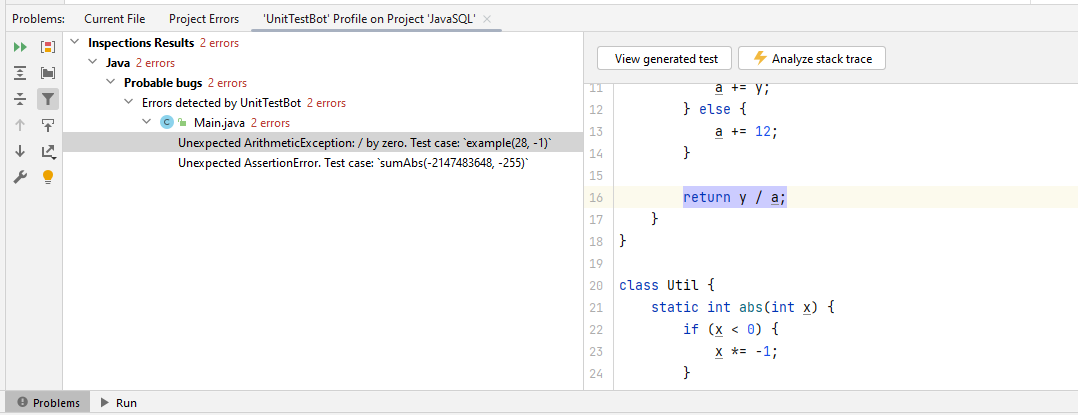
\includegraphics{images/problems-view.png}
}
\caption{
\label{problems-view} Интерфейс просмотра результатов статического анализа.}
\end{flushleft}
\end{figure}

\begin{figure}[ht]
\begin{flushleft}
\scalebox{0.55}{
   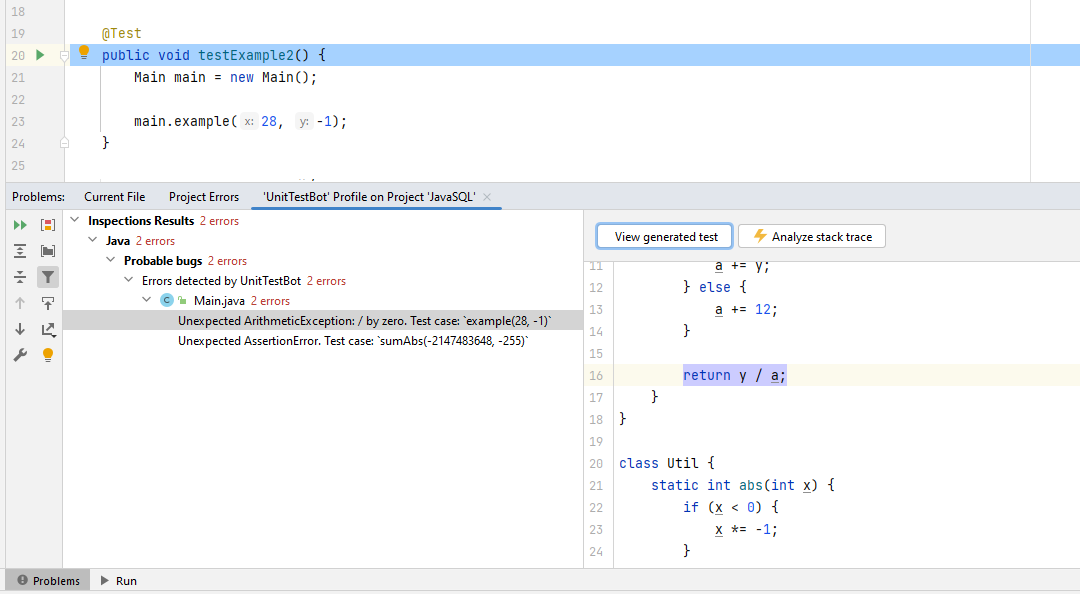
\includegraphics{images/problems-view-test.png}
}
\caption{
\label{problems-view-test} Ссылка на сгенерированный тест.}
\end{flushleft}
\end{figure}

\begin{figure}[ht]
\begin{flushleft}
\scalebox{0.55}{
   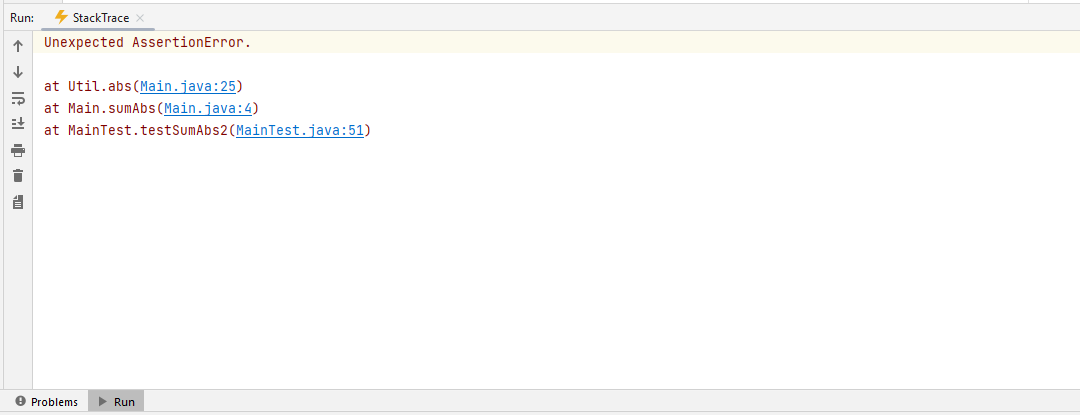
\includegraphics{images/problems-view-stacktrace.png}
}
\caption{
\label{problems-view-stacktrace} Просмотр трассировки стека.}
\end{flushleft}
\end{figure}

\begin{figure}[ht]
\begin{flushleft}
\scalebox{0.55}{
   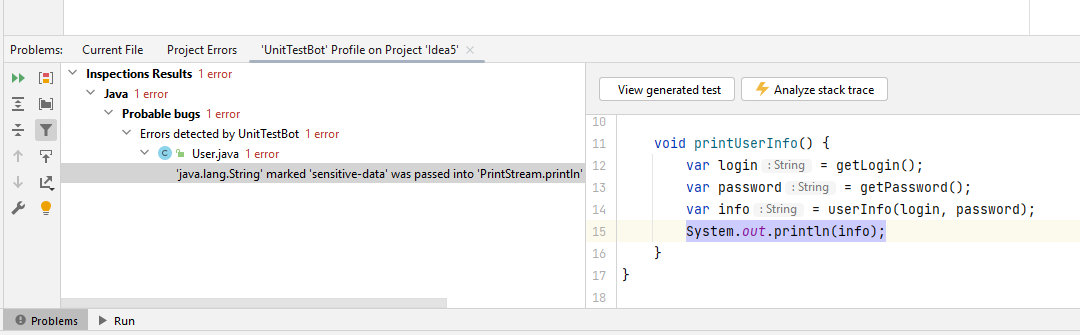
\includegraphics{images/problems-view-taint.png}
}
\caption{
\label{problems-view-taint} Обнаруженная taint-анализом проблема.}
\end{flushleft}
\end{figure}

\definecolor{error-red}{rgb}{1.0, 0.8, 0.8}

\begin{listing}[ht]
\begin{minted}[highlightlines={24},highlightcolor=error-red,linenos,baselinestretch=1,style=abap]{java}
public static int solve(String s) {
    for (int i = 0; i < s.length(); ++i) {
        assume('a' <= s.charAt(i) && s.charAt(i) <= 'z');
    }

    int counter = 0;
    int count = 0;
    while (count < s.length()) {
        counter++;
        char mem1 = s.charAt(count++);
        while (count < s.length() && s.charAt(count) == mem1) {
            count++;
        }
        if (count >= s.length()) {
            break;
        }
        char mem2 = s.charAt(count++);
        while (
            count < s.length() && (s.charAt(count) == mem1 || 
            s.charAt(count) == mem2)
        ) {
            count++;
        }
        char mem3 = s.charAt(count++);
        while (
            count < s.length() && (s.charAt(count) == mem1 || 
            s.charAt(count) == mem2 || s.charAt(count) == mem3)
        ) {
            count++;
        }
    }

    return counter;
}
\end{minted}
\caption{Решение задачи Codeforces-805B, в котором допущена ошибка.}
\label{cf-example}
\end{listing}


\end{document}
